This section distinguishes the kinds of editorial problems the gardener can resolve locally from the kinds that require specialist handoff. Not every defect in a draft is the same defect: some passages repeat an idea that has already been established, some move too abruptly between claims, some introduce a term that has not yet been defined, and some assert a fact that the manuscript does not yet support. The maintenance cycle in Section~5.1 treats these as different signals because they route to different agents and different repair strategies.

Repeated claims are usually the easiest to detect. When two adjacent sections restate the same point in nearly the same language, the problem is not factual correctness but redundancy. The gardener can mark the overlap and ask the relevant section agent to compress or remove the repeated material. In practice, this is a local revision request: the section agent revises its own payload so the manuscript keeps one clear statement instead of several near-duplicates. The goal is not to eliminate all reinforcement, but to avoid prose that feels circular or padded.

Thin transitions are a related but distinct issue. A section may be individually correct and still read as if one paragraph has been pasted next to another without connective tissue. In that case, the gardener does not ask for new evidence; it asks for a better bridge. The section agent may need to add a sentence that explains why the next concept follows from the previous one, or to restate the local purpose of the section so the reader can track the argument. These requests are editorial rather than substantive: they improve continuity, pacing, and reader orientation without changing the underlying claim.

Missing definitions require a different response. If a section uses a term that the outline or surrounding prose has not yet defined, the gardener should not let the term drift into vague usage. Instead, it routes the issue back to the section agent responsible for the local context, or to the section that owns the concept if the definition belongs elsewhere in the outline. The repair may be as simple as adding a short definition where the term first appears, or as involved as coordinating with a sibling section so the definition is introduced before the term is reused. The important point is that undefined terminology is a structural gap, not merely a stylistic flaw.

Unsupported assertions are the category that most clearly requires reference support. When a section makes a claim that depends on external evidence, implementation details, or a specific documented behavior, the gardener checks whether the manuscript already has a registered citation key that can support it. If the claim is already backed by a registered source, the section agent can cite it directly. If not, the issue is escalated to \texttt{references\_agent} through a structured request for research or citation registration. The section agent should not invent a citation key or leave a fabricated reference in place. It should either wait for the registered key or revise the prose so that it no longer overstates what the manuscript can currently support.

These categories route differently because they imply different kinds of repair. Repetition and thin transitions are usually handled by the owning section agent, since they are matters of local prose shape. Missing definitions may also be handled locally, but they often require coordination with a sibling section or an earlier chapter if the definition belongs in a shared conceptual foundation. Unsupported assertions, by contrast, are routed toward \texttt{references\_agent} whenever the manuscript needs a source that is not yet registered. That handoff preserves the separation between prose revision and bibliography ownership.

The gardener's job is therefore not simply to flag problems, but to classify them. A repeated claim asks for compression. A thin transition asks for connective prose. A missing definition asks for conceptual repair. An unsupported assertion asks for citation support or for the claim to be softened until support exists. By separating these cases, the editorial loop keeps revision requests precise, keeps section agents focused on the work they own, and keeps \texttt{references\_agent} responsible for the evidence trail that underwrites the manuscript.

In the broader maintenance cycle, this classification also prevents unnecessary escalation. A section that merely repeats itself does not need a bibliography search. A section that lacks a definition does not need a global rewrite. And a claim that lacks support should not be disguised as a stylistic issue. The manuscript stays coherent when each defect is routed to the agent best suited to repair it, and this section names the routing logic that makes that possible.

A useful way to read the gardener's classification is as a small decision tree. If the text says the same thing twice, the fix is compression. If the text jumps too quickly, the fix is a transition. If the text uses a term before the reader can place it, the fix is a definition or a coordination request. If the text reaches beyond what the manuscript can currently justify, the fix is either a citation or a more cautious claim. That distinction matters because it keeps editorial work proportional: the gardener does not turn every problem into a research task, and it does not turn every research need into a prose-only edit.

This routing logic also makes revision requests easier to interpret downstream. A section agent receiving a note about repetition knows to shorten or merge material. A note about a thin transition tells the agent to add connective prose rather than new content. A note about a missing definition signals that the section may need to borrow conceptual groundwork from a sibling or earlier section. And a note about an unsupported assertion tells the agent to either cite a registered source or narrow the claim until support is available. The request itself therefore carries the repair strategy, which reduces ambiguity and keeps the editorial loop efficient.

Taken together, these checks show that gardening is not a generic quality filter. It is a classification layer that separates prose shape, conceptual completeness, and evidentiary support. That separation is what lets the system route work to the right owner: section agents handle local revision, sibling coordination resolves shared terminology, and \texttt{references\_agent} owns the evidence trail. The result is a manuscript that can be corrected without collapsing every issue into the same kind of task.

One practical implication is that the gardener can keep a revision note narrowly scoped. If the problem is repetition, the note can point to the duplicated sentence and ask for compression. If the problem is a thin transition, the note can ask for one bridging sentence rather than a wholesale rewrite. If the problem is a missing definition, the note can identify the first occurrence of the term and ask whether the definition belongs here or in a sibling section. If the problem is an unsupported assertion, the note can either request a registered citation or ask the authoring agent to soften the claim until support is available. That specificity keeps the maintenance cycle efficient and reduces the chance that a local issue becomes a broad editorial detour.

In the context of this chapter, the section also sets up the next distinction: local editorial checks versus manuscript-level drift. The checks described here are the ones the gardener can usually resolve by targeting a single section or a small set of related sections. When the same issue spans multiple sections, the problem is no longer just a revision request; it becomes a coordination problem for the hypervisor. Section~5.3 takes up that broader escalation path.

\begin{figure}[htbp]
\centering
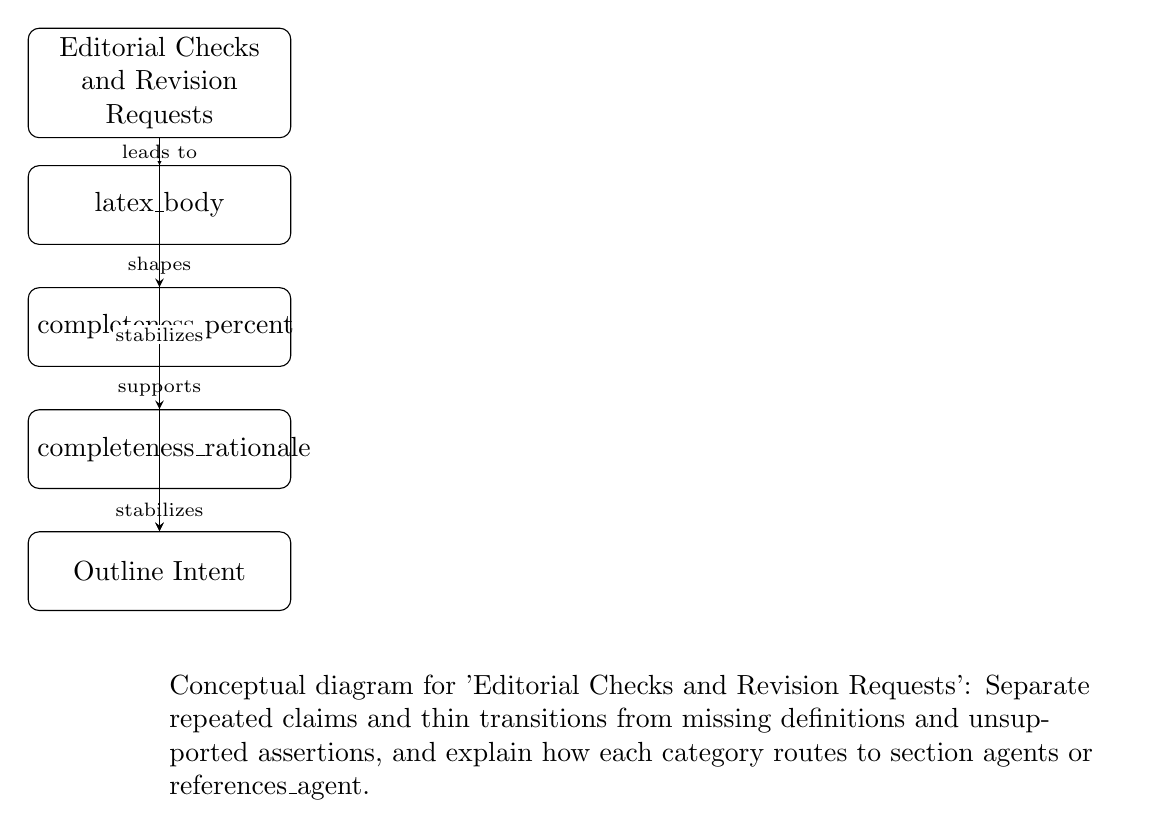
\begin{tikzpicture}[>=stealth, node distance=2.2cm,
  concept/.style={draw, rounded corners, align=center, text width=3.1cm, minimum height=1cm},
  relation/.style={font=\scriptsize, fill=white, inner sep=1pt}]
\node[concept] (n1) at (0,0.0) {Editorial Checks and Revision Requests};
\node[concept] (n2) at (0,-1.55) {latex\_body};
\node[concept] (n3) at (0,-3.1) {completeness\_percent};
\node[concept] (n4) at (0,-4.65) {completeness\_rationale};
\node[concept] (n5) at (0,-6.2) {Outline Intent};
\draw[->] (n1) -- node[relation] {leads to} (n2);
\draw[->] (n2) -- node[relation] {shapes} (n3);
\draw[->] (n3) -- node[relation] {supports} (n4);
\draw[->] (n4) -- node[relation] {stabilizes} (n5);
\draw[->] (n1) -- node[relation] {stabilizes} (n5);
\node[align=left, text width=12cm, anchor=north west] at (0,-7.4) {Conceptual diagram for 'Editorial Checks and Revision Requests': Separate repeated claims and thin transitions from missing definitions and unsupported assertions, and explain how each category routes to section agents or references\_agent.};
\end{tikzpicture}

\caption{Conceptual diagram for ``Editorial Checks and Revision Requests'': separate repeated claims and thin transitions from missing definitions and unsupported assertions, and show how each category routes to section agents or \texttt{references\_agent}.}
\end{figure}
